\documentclass[a4paper,titlepage]{article}
\usepackage[utf8]{inputenc}   % pro unicode UTF-8
\usepackage[czech]{babel} %jazyk dokumentu
\usepackage{listings}
\usepackage{color}
\usepackage[T1]{fontenc}
\usepackage{hyperref}
\usepackage{listingsutf8}
\usepackage{graphicx}
\usepackage{lipsum}
\usepackage{amssymb}
\usepackage{geometry}


 \geometry{
 a4paper,
 left=30mm,
 top=20mm,
 }

\graphicspath{ {/} }

\title{}
\author{David Nápravník}
\date{2018}

%%%%%%%%%%%%%%%%%%%%%%%%%%%%%%%%%%%%%%%%%%%%%%%%%%%%%%%%%%%%%

\begin{document}
\noindent E. Zápočtový test - MA I. (2.2.2018) \\
David Nápravník\\
\\
\section{Spočítejte limitu (n $\in \mathbb{N} $)}
$$
	\lim_{n \to \infty}\frac{(n +\frac{2}{n})^5}{(2n - \frac{1}{n})^6}*\sqrt{2n+3}*\sqrt{3n+2}
$$
Nejdříve spojíme vše do jednoho zlomku
$$
	\lim_{n \to \infty}\frac{(n +\frac{2}{n})^5*\sqrt{2n+3}*\sqrt{3n+2}}{(2n - \frac{1}{n})^6}
$$
Jelikož n $\to \infty $ tak $ \frac{2}{n} = 0 $ a $ \frac{1}{n} = 0 $
$$
	\lim_{n \to \infty}\frac{(n + 0)^5*\sqrt{2n+3}*\sqrt{3n+2}}{(2n - 0)^6}
$$
$(2n)^6 = 64 n^6$ a to rovnou zkrátíme s $n^5$
$$
	\lim_{n \to \infty}\frac{\sqrt{2n+3}*\sqrt{3n+2}}{64n}
$$
Převedeme pod společný zlomek
$$
	\lim_{n \to \infty}\sqrt{\frac{(2n+3)*(3n+2)}{(64n)^2}}
$$
Posuneme limitu dovnitř mocniny a vytkneme spodek zlomku
$$
	\sqrt{\frac{1}{64^2}\lim_{n \to \infty}{\frac{(2n+3)*(3n+2)}{n^2}}}
$$
Vypočítáme zlomek
$$
	\sqrt{\frac{1}{64^2}\lim_{n \to \infty}{\frac{6n^2+13n+6}{n^2}}}
$$
Použijeme L'Hospitala, protože máme $ \frac{\infty}{\infty}$
$$
	\sqrt{\frac{1}{64^2}\lim_{n \to \infty}{\frac{12n+13}{2n}}}
$$
Vykrátíme $n$
$$
	\sqrt{\frac{1}{64^2}\lim_{n \to \infty}{\frac{12+\frac{13}{n}}{2}}}
$$
Vypočítáme limitu
$$
	\sqrt{\frac{1}{64^2}*{\frac{12}{2}}} = \frac{\sqrt{\frac{3}{2}}}{32}
$$





\section{Mějme následující číselnou řadu.}
$$
\sum^{\infty}_{n=1}\frac{3^n+(-1)^n*2^n*n}{4^n + (-1)^n*n}
$$
Podíváme se zda $\lim a_n = 0$
$$
\lim_{n\to \infty}\frac{3^n+(-1)^n*2^n*n}{4^n + (-1)^n*n}
$$
Pro a >> 1 $ \lim_{n\to \infty} a^n > \lim_{n\to \infty} n $\\
A jelikož $4^n >> 3^n + 2^n$ tak
$$
\lim_{n\to \infty}\frac{3^n}{4^n} = 0
$$
Srovnávacím kritériem můžeme odstranit $(-1)^n$ 
$$
\sum^{\infty}_{n=1}\frac{3^n+2^n*n}{4^n + n}  \geq 
\sum^{\infty}_{n=1}\frac{3^n-2^n*n}{4^n - n}
$$
jelikož se nedostaneme do záporných hodnot tak pokud nastane neabsolutní konvergence bude zároveň i absolutní.\\
\\
Dále vypočítáme konvergenci a jelikož $3^n > 2^n*n$ a zároveň $4^n > n$
$$
\sum^{\infty}_{n=1}\frac{3^n+2^n*n}{4^n + n}
$$
Srovnávacím kritériem
$$
\sum^{\infty}_{n=1}\frac{3^n+2^n*n}{4^n + n} \leq
\sum^{\infty}_{n=1}\frac{3^n + 2^n*n}{4^n}
$$
zkontrolujeme konvergenci pro pravou řadu\\
$$
\sum^{\infty}_{n=1}\frac{3^n + 2^n*n}{4^n}=
\sum^{\infty}_{n=1}\frac{3^n}{4^n}+
\sum^{\infty}_{n=1}\frac{2^n*n}{4^n}
$$
Odmocninovým kritériem:
$$
k_1 = \sqrt[n]{\frac{3^n}{4^n}} = 3/4 
$$ $$
k_2 = \sqrt[n]{\frac{2^n*n}{4^n}} = \sqrt[n]{\frac{2^n}{4^n}} * \sqrt[n]{n} = \frac{2*1}{4} = 2/4 \qquad\qquad \lim_{n \to \infty}\sqrt[n]{n} = 1
$$
pokud je $k<1$ pak řada konverguje.
Takže jelikož obě řady konvergují, tak i jejich součet bude konvergovat.
Takže platí srovnávací kritérium a tudíž původní řada \textbf{konverguje absolutně i neabsolutně}.






\section{Mějme funkci f}
$$
f(x)=\sin^2 \sqrt{\frac{x^2-1}{x}}
$$
Kritické body:\\
$ x \neq 0 $ kvůli zlomku\\
$ x > 1 $ kvůli odmocnině\\
\\
Definiční obor: $x \in \langle -1,0 ) \cup \langle 1,\infty )$ (bez použití komplexních čísel).\\
Funkce je spojitá na daném definičním oboru. (protože kritický bod x=0 se nenachází v daném definičním oboru)\\
\\
Derivace:
$$
f(x)'=\frac{	(2-\frac{x^2-1}{x^2})	\sin \sqrt{\frac{x^2-1}{x}}\cos \sqrt{\frac{x^2-1}{x}}}{\sqrt{\frac{x^2-1}{x}}}
$$
kritickými body derivace jsou:\\
$x = \pm 1$\\
$x= 0$\\
\\
pro $x \in ( -1,0 ) \cup (1,\infty)$ existuje derivace f(x)'\\
\\
Jednostranné derivace: pro $x = 1$
$$
\frac{	\sin \sqrt{\frac{x^2-1}{x}}}{\sqrt{\frac{x^2-1}{x}}} = \frac{\sin j}{j} = 1, j = \sqrt{\frac{x^2-1}{x}}
$$
Po vykrácení sin a jmenovatele nám zbude:
$$
\lim_{x \to 1}(2-\frac{x^2-1}{x^2})\cos \sqrt{\frac{x^2-1}{x}} \stackrel{VOAL}{=} (2-0) * 1 = 2
$$
Derivace pro x = -1
$$
\lim_{x \to -1}(2-\frac{x^2-1}{x^2})\cos \sqrt{\frac{x^2-1}{x}} \stackrel{VOAL}{=} (2-0) * 1 = 2
$$







\section{Vyšetřete průběh funkce f}
$$
f(x)=exp(\frac{x-1}{x})
$$
kritické body:\\
$x = 0$\\
spočítáme limity zprava,zleva kolem nuly a pak limity do nekonečna
$$
\lim_{n \to 0^+}exp(\frac{x-1}{x})
$$ $$
\lim_{n \to 0^+}exp(1-\frac{1}{x}) \stackrel{VOAL}{=} e^{1-\infty} = e^{-\infty} = 0
$$ 

$$
\lim_{n \to 0^-}exp(\frac{x-1}{x})
$$ $$
\lim_{n \to 0^-}exp(1-\frac{1}{x}) \stackrel{VOAL}{=} exp(1-(\frac{1}{-0})) = exp(1-(-\infty))  = e^{\infty} = \infty
$$ 

$$
\lim_{n \to \infty}exp(\frac{x-1}{x})
$$ $$
\lim_{n \to \infty}exp(1-\frac{1}{x}) \stackrel{VOAL}{=} exp(1-(\frac{1}{\infty})) = exp(1-(0))  = e^{1} = e
$$ 

$$
\lim_{n \to -\infty}exp(\frac{x-1}{x})
$$ $$
\lim_{n \to -\infty}exp(1-\frac{1}{x}) \stackrel{VOAL}{=} exp(1-(\frac{1}{-\infty})) = exp(1-(-0))  = e^{1} = e
$$ 
Najdeme kdy se derivace rovná nule.\\
$$ f(x)' = \frac{e^{1-\frac{1}{x}}}{x^2} $$
$$ exp(1-\frac{1}{y}) = 0, y \in \emptyset$$
jelikož funkce nemá derivaci rovnou nule tak nenabývá lokálního maxima ani minima\\
\\
pro $ a \in \mathbb{R}  e^a > 0 \to $ derivace je nezáporná $\to$ původní funkce je na celém DO rostoucí\\
\\
funkce nemá globální maximum ani minimum\\
funkce nemá lokální maximum ani minimum
\begin{figure}[h]
	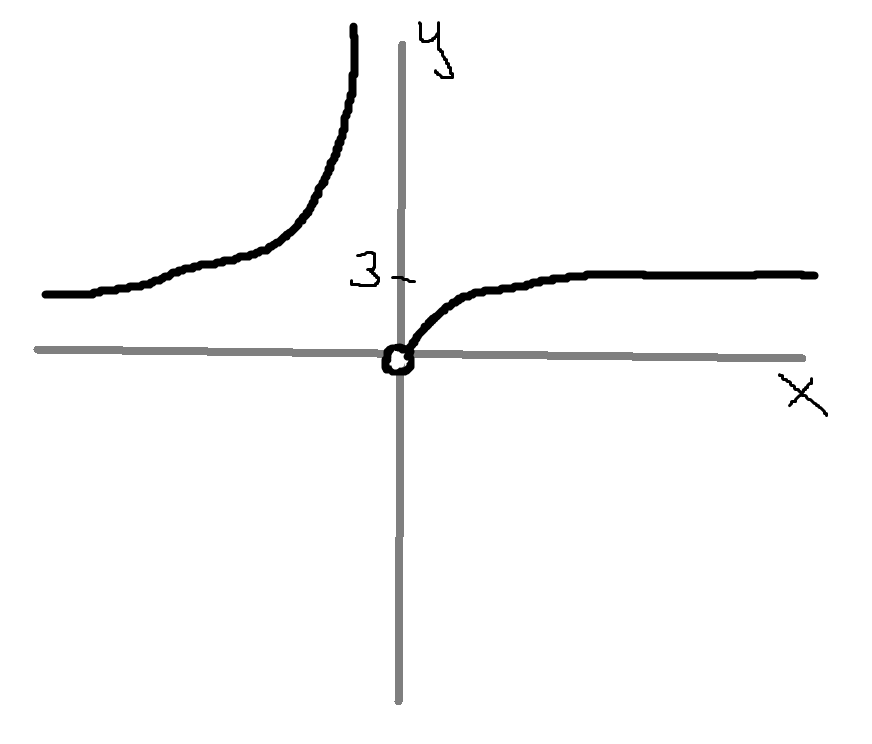
\includegraphics[scale=0.2]{graf_1_zapocet_mataliza.png}
\end{figure}













\end{document}